\documentclass{article}
\usepackage[table]{xcolor}
\usepackage{array}
\usepackage{float}
\usepackage{graphicx}
\usepackage{tikz}
\usepackage{tcolorbox}
\usepackage{amsmath}

\renewcommand\thesubsection{\arabic{subsection}} % Hace que subsección use solo números (1, 2, 3, etc.)
\setcounter{secnumdepth}{2} % Asegura que las subsecciones se numerarán

\title{AULA5: Exercício teórico métodos de ordenação lineares}
\author{Aluno: Gian Franco Joel Condori Luna}
\date{\today}

\begin{document}

\maketitle

\section*{Exercices}
\setcounter{section}{1}
\subsection {(0,3) Ilustre a ordenação por contagem sobre o vetor \\ 
A = [ 6, 0, 2, 0, 1, 3 , 4, 6, 1, 3, 2].}

\subsubsection{Solução:}

\[
C = \quad
\begin{array}{|c|c|c|c|c|c|c|}
\hline
2 & 2 & 2 & 2 & 1 & 0 & 2 \\ 
\hline
\end{array}
\]

\[
C = \quad
\begin{array}{|c|c|c|c|c|c|c|}
\hline
2 & 4 & 6 & 8 & 9 & 9 & 11 \\ 
\hline
\end{array}
\]

\begin{center}
    \begin{tikzpicture}
        \draw[thick] (0,0) -- (3,0); % Línea antes del texto
        \node[anchor=mid] at (5,0) {\Large n = 11}; % Texto centrado
        \draw[thick] (6.5,0) -- (9.5,0); % Línea después del texto
    \end{tikzpicture}
\end{center}

\[
A = \quad
\begin{array}{|c|c|c|c|c|c|c|c|c|c|c|}
\hline
6 & 0 & 2 & 0 & 1 & 3 & 4 & 6 & 1 & 3 & \textcolor{red}{2} \\ 
\hline
\end{array}
\]

\[
C = \quad
\begin{array}{|c|c|c|c|c|c|c|}
\hline
2 & 4 & \textcolor{red}{6} & 8 & 9 & 9 & 11 \\ 
\hline
\end{array}
\]

\[
B = \quad
\begin{array}{|c|c|c|c|c|c|c|c|c|c|c|}
\hline
\cellcolor{gray}{} & \cellcolor{gray}{} & \cellcolor{gray}{} & \cellcolor{gray}{} & \cellcolor{gray}{} & 2 & \cellcolor{gray}{} & \cellcolor{gray}{} & \cellcolor{gray}{} & \cellcolor{gray}{} & \cellcolor{gray}{} \\ 
\hline
\end{array}
\]

\[
C = \quad
\begin{array}{|c|c|c|c|c|c|c|}
\hline
2 & 4 & 5 & 8 & 9 & 9 & 11 \\ 
\hline
\end{array}
\]


\begin{center}
    \begin{tikzpicture}
        \draw[thick] (0,0) -- (3,0); % Línea antes del texto
        \node[anchor=mid] at (5,0) {\Large n = 10}; % Texto centrado
        \draw[thick] (6.5,0) -- (9.5,0); % Línea después del texto
    \end{tikzpicture}
\end{center}

\[
A = \quad
\begin{array}{|c|c|c|c|c|c|c|c|c|c|c|}
\hline
6 & 0 & 2 & 0 & 1 & 3 & 4 & 6 & 1 & \textcolor{red}{3} & 2 \\ 
\hline
\end{array}
\]

\[
C = \quad
\begin{array}{|c|c|c|c|c|c|c|}
\hline
2 & 4 & 5 & \textcolor{red}{8} & 9 & 9 & 11 \\ 
\hline
\end{array}
\]

\[
B = \quad
\begin{array}{|c|c|c|c|c|c|c|c|c|c|c|}
\hline
\cellcolor{gray}{} & \cellcolor{gray}{} & \cellcolor{gray}{} & 
\cellcolor{gray}{} & \cellcolor{gray}{} & 2 & 
\cellcolor{gray}{} & 3 & \cellcolor{gray}{} & 
\cellcolor{gray}{} & \cellcolor{gray}{} \\ 
\hline
\end{array}
\]

\[
C = \quad
\begin{array}{|c|c|c|c|c|c|c|}
\hline
2 & 4 & 5 & 7 & 9 & 9 & 11 \\ 
\hline
\end{array}
\]


\begin{center}
    \begin{tikzpicture}
        \draw[thick] (0,0) -- (3,0); % Línea antes del texto
        \node[anchor=mid] at (5,0) {\Large n = 9}; % Texto centrado
        \draw[thick] (6.5,0) -- (9.5,0); % Línea después del texto
    \end{tikzpicture}
\end{center}

\[
A = \quad
\begin{array}{|c|c|c|c|c|c|c|c|c|c|c|}
\hline
6 & 0 & 2 & 0 & 1 & 3 & 4 & 6 & \textcolor{red}{1} & 3 & 2 \\ 
\hline
\end{array}
\]

\[
C = \quad
\begin{array}{|c|c|c|c|c|c|c|}
\hline
2 & \textcolor{red}{4} & 5 & 7 & 9 & 9 & 11 \\ 
\hline
\end{array}
\]

\[
B = \quad
\begin{array}{|c|c|c|c|c|c|c|c|c|c|c|}
\hline
\cellcolor{gray}{} & \cellcolor{gray}{} & \cellcolor{gray}{} & 
1 & \cellcolor{gray}{} & 2 & 
\cellcolor{gray}{} & 3 & \cellcolor{gray}{} & 
\cellcolor{gray}{} & \cellcolor{gray}{} \\ 
\hline
\end{array}
\]

\[
C = \quad
\begin{array}{|c|c|c|c|c|c|c|}
\hline
2 & 3 & 5 & 7 & 9 & 9 & 11 \\ 
\hline
\end{array}
\]


\begin{center}
    \begin{tikzpicture}
        \draw[thick] (0,0) -- (3,0); % Línea antes del texto
        \node[anchor=mid] at (5,0) {\Large n = 8}; % Texto centrado
        \draw[thick] (6.5,0) -- (9.5,0); % Línea después del texto
    \end{tikzpicture}
\end{center}

\[
A = \quad
\begin{array}{|c|c|c|c|c|c|c|c|c|c|c|}
\hline
6 & 0 & 2 & 0 & 1 & 3 & 4 & \textcolor{red}{6} & 1 & 3 & 2 \\ 
\hline
\end{array}
\]

\[
C = \quad
\begin{array}{|c|c|c|c|c|c|c|}
\hline
2 & 3 & 5 & 7 & 9 & 9 & \textcolor{red}{11} \\ 
\hline
\end{array}
\]

\[
B = \quad
\begin{array}{|c|c|c|c|c|c|c|c|c|c|c|}
\hline
\cellcolor{gray}{} & \cellcolor{gray}{} & \cellcolor{gray}{} & 
1 & \cellcolor{gray}{} & 2 & 
\cellcolor{gray}{} & 3 & \cellcolor{gray}{} & 
\cellcolor{gray}{} & 6 \\ 
\hline
\end{array}
\]

\[
C = \quad
\begin{array}{|c|c|c|c|c|c|c|}
\hline
2 & 3 & 5 & 7 & 9 & 9 & 10 \\ 
\hline
\end{array}
\]


\begin{center}
    \begin{tikzpicture}
        \draw[thick] (0,0) -- (3,0); % Línea antes del texto
        \node[anchor=mid] at (5,0) {\Large n = 7}; % Texto centrado
        \draw[thick] (6.5,0) -- (9.5,0); % Línea después del texto
    \end{tikzpicture}
\end{center}

\[
A = \quad
\begin{array}{|c|c|c|c|c|c|c|c|c|c|c|}
\hline
6 & 0 & 2 & 0 & 1 & 3 & \textcolor{red}{4} & 6 & 1 & 3 & 2 \\ 
\hline
\end{array}
\]

\[
C = \quad
\begin{array}{|c|c|c|c|c|c|c|}
\hline
2 & 3 & 5 & 7 & \textcolor{red}{9} & 9 & 10 \\ 
\hline
\end{array}
\]

\[
B = \quad
\begin{array}{|c|c|c|c|c|c|c|c|c|c|c|}
\hline
\cellcolor{gray}{} & \cellcolor{gray}{} & \cellcolor{gray}{} & 
1 & \cellcolor{gray}{} & 2 & 
\cellcolor{gray}{} & 3 & 4 & 
\cellcolor{gray}{} & 6 \\ 
\hline
\end{array}
\]

\[
C = \quad
\begin{array}{|c|c|c|c|c|c|c|}
\hline
2 & 3 & 5 & 7 & 8 & 9 & 10 \\ 
\hline
\end{array}
\]


\begin{center}
    \begin{tikzpicture}
        \draw[thick] (0,0) -- (3,0); % Línea antes del texto
        \node[anchor=mid] at (5,0) {\Large n = 6}; % Texto centrado
        \draw[thick] (6.5,0) -- (9.5,0); % Línea después del texto
    \end{tikzpicture}
\end{center}

\[
A = \quad
\begin{array}{|c|c|c|c|c|c|c|c|c|c|c|}
\hline
6 & 0 & 2 & 0 & 1 & \textcolor{red}{3} & 4 & 6 & 1 & 3 & 2 \\ 
\hline
\end{array}
\]

\[
C = \quad
\begin{array}{|c|c|c|c|c|c|c|}
\hline
2 & 3 & 5 & \textcolor{red}{7} & 8 & 9 & 10 \\ 
\hline
\end{array}
\]

\[
B = \quad
\begin{array}{|c|c|c|c|c|c|c|c|c|c|c|}
\hline
\cellcolor{gray}{} & \cellcolor{gray}{} & \cellcolor{gray}{} & 
1 & \cellcolor{gray}{} & 2 & 
3 & 3 & 4 & 
\cellcolor{gray}{} & 6 \\ 
\hline
\end{array}
\]

\[
C = \quad
\begin{array}{|c|c|c|c|c|c|c|}
\hline
2 & 3 & 5 & 6 & 8 & 9 & 10 \\ 
\hline
\end{array}
\]


\begin{center}
    \begin{tikzpicture}
        \draw[thick] (0,0) -- (3,0); % Línea antes del texto
        \node[anchor=mid] at (5,0) {\Large n = 5}; % Texto centrado
        \draw[thick] (6.5,0) -- (9.5,0); % Línea después del texto
    \end{tikzpicture}
\end{center}

\[
A = \quad
\begin{array}{|c|c|c|c|c|c|c|c|c|c|c|}
\hline
6 & 0 & 2 & 0 & \textcolor{red}{1} & 3 & 4 & 6 & 1 & 3 & 2 \\ 
\hline
\end{array}
\]

\[
C = \quad
\begin{array}{|c|c|c|c|c|c|c|}
\hline
2 & \textcolor{red}{3} & 5 & 6 & 8 & 9 & 10 \\ 
\hline
\end{array}
\]

\[
B = \quad
\begin{array}{|c|c|c|c|c|c|c|c|c|c|c|}
\hline
\cellcolor{gray}{} & \cellcolor{gray}{} & 1 & 
1 & \cellcolor{gray}{} & 2 & 
3 & 3 & 4 & 
\cellcolor{gray}{} & 6 \\ 
\hline
\end{array}
\]

\[
C = \quad
\begin{array}{|c|c|c|c|c|c|c|}
\hline
2 & 2 & 5 & 6 & 8 & 9 & 10 \\ 
\hline
\end{array}
\]

\begin{center}
    \begin{tikzpicture}
        \draw[thick] (0,0) -- (3,0); % Línea antes del texto
        \node[anchor=mid] at (5,0) {\Large n = 4}; % Texto centrado
        \draw[thick] (6.5,0) -- (9.5,0); % Línea después del texto
    \end{tikzpicture}
\end{center}

\[
A = \quad
\begin{array}{|c|c|c|c|c|c|c|c|c|c|c|}
\hline
6 & 0 & 2 & \textcolor{red}{0} & 1 & 3 & 4 & 6 & 1 & 3 & 2 \\ 
\hline
\end{array}
\]

\[
C = \quad
\begin{array}{|c|c|c|c|c|c|c|}
\hline
\textcolor{red}{2} & 2 & 5 & 6 & 8 & 9 & 10 \\ 
\hline
\end{array}
\]

\[
B = \quad
\begin{array}{|c|c|c|c|c|c|c|c|c|c|c|}
\hline
\cellcolor{gray}{} & 0 & 1 & 
1 & \cellcolor{gray}{} & 2 & 
3 & 3 & 4 & 
\cellcolor{gray}{} & 6 \\ 
\hline
\end{array}
\]

\[
C = \quad
\begin{array}{|c|c|c|c|c|c|c|}
\hline
1 & 2 & 5 & 6 & 8 & 9 & 10 \\ 
\hline
\end{array}
\]


\begin{center}
    \begin{tikzpicture}
        \draw[thick] (0,0) -- (3,0); % Línea antes del texto
        \node[anchor=mid] at (5,0) {\Large n = 3}; % Texto centrado
        \draw[thick] (6.5,0) -- (9.5,0); % Línea después del texto
    \end{tikzpicture}
\end{center}

\[
A = \quad
\begin{array}{|c|c|c|c|c|c|c|c|c|c|c|}
\hline
6 & 0 & \textcolor{red}{2} & 0 & 1 & 3 & 4 & 6 & 1 & 3 & 2 \\ 
\hline
\end{array}
\]

\[
C = \quad
\begin{array}{|c|c|c|c|c|c|c|}
\hline
1 & 2 & \textcolor{red}{5} & 6 & 8 & 9 & 10 \\ 
\hline
\end{array}
\]

\[
B = \quad
\begin{array}{|c|c|c|c|c|c|c|c|c|c|c|}
\hline
\cellcolor{gray}{} & 0 & 1 & 
1 & 2 & 2 & 
3 & 3 & 4 & 
\cellcolor{gray}{} & 6 \\ 
\hline
\end{array}
\]

\[
C = \quad
\begin{array}{|c|c|c|c|c|c|c|}
\hline
1 & 2 & 4 & 6 & 8 & 9 & 10 \\ 
\hline
\end{array}
\]

\begin{center}
    \begin{tikzpicture}
        \draw[thick] (0,0) -- (3,0); % Línea antes del texto
        \node[anchor=mid] at (5,0) {\Large n = 2}; % Texto centrado
        \draw[thick] (6.5,0) -- (9.5,0); % Línea después del texto
    \end{tikzpicture}
\end{center}

\[
A = \quad
\begin{array}{|c|c|c|c|c|c|c|c|c|c|c|}
\hline
6 & \textcolor{red}{0} & 2 & 0 & 1 & 3 & 4 & 6 & 1 & 3 & 2 \\ 
\hline
\end{array}
\]

\[
C = \quad
\begin{array}{|c|c|c|c|c|c|c|}
\hline
\textcolor{red}{1} & 2 & 4 & 6 & 8 & 9 & 10 \\ 
\hline
\end{array}
\]

\[
B = \quad
\begin{array}{|c|c|c|c|c|c|c|c|c|c|c|}
\hline
0 & 0 & 1 & 
1 & 2 & 2 & 
3 & 3 & 4 & 
\cellcolor{gray}{} & 6 \\ 
\hline
\end{array}
\]

\[
C = \quad
\begin{array}{|c|c|c|c|c|c|c|}
\hline
0 & 2 & 4 & 6 & 8 & 9 & 10 \\ 
\hline
\end{array}
\]


\begin{center}
    \begin{tikzpicture}
        \draw[thick] (0,0) -- (3,0); % Línea antes del texto
        \node[anchor=mid] at (5,0) {\Large n = 1}; % Texto centrado
        \draw[thick] (6.5,0) -- (9.5,0); % Línea después del texto
    \end{tikzpicture}
\end{center}

\[
A = \quad
\begin{array}{|c|c|c|c|c|c|c|c|c|c|c|}
\hline
\textcolor{red}{6} & 0 & 2 & 0 & 1 & 3 & 4 & 6 & 1 & 3 & 2 \\ 
\hline
\end{array}
\]

\[
C = \quad
\begin{array}{|c|c|c|c|c|c|c|}
\hline
0 & 2 & 4 & 6 & 8 & 9 & \textcolor{red}{10} \\ 
\hline
\end{array}
\]

\[
B = \quad
\begin{array}{|c|c|c|c|c|c|c|c|c|c|c|}
\hline
0 & 0 & 1 & 
1 & 2 & 2 & 
3 & 3 & 4 & 
6 & 6 \\ 
\hline
\end{array}
\]

\[
C = \quad
\begin{array}{|c|c|c|c|c|c|c|}
\hline
0 & 2 & 4 & 6 & 8 & 9 & 9 \\ 
\hline
\end{array}
\]

\begin{tcolorbox}[title=Resposta, colframe=black, colback=white] % Personaliza el color del marco y del fondo
    \[
    B = \quad
    \begin{array}{|c|c|c|c|c|c|c|c|c|c|c|}
    \hline
    0 & 0 & 1 & 
    1 & 2 & 2 & 
    3 & 3 & 4 & 
    6 & 6 \\ 
    \hline
    \end{array}
    \]
\end{tcolorbox}

\subsection {(0,3) Ilustre a ordenação radix-sort sobre a seguinte lista de palavras: cow, dog, sea,
rug, row, mob, box, tab, bar, ear, tar, dig, big, tea, now, fox.}

\subsubsection{Solução:}


\begin{center}
    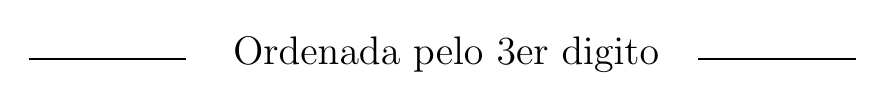
\begin{tikzpicture}
        \draw[thick] (0,0) -- (2,0); % Línea antes del texto
        \node[anchor=mid] at (5.3,0) {\Large Ordenada pelo 3er digito}; % Texto centrado
        \draw[thick] (8.5,0) -- (10.5,0); % Línea después del texto
    \end{tikzpicture}
\end{center}
\begin{center}
    co\textcolor{red}{w}, do\textcolor{red}{g}, se\textcolor{red}{a}, ru\textcolor{red}{g}, ro\textcolor{red}{w}, mo\textcolor{red}{b}, bo\textcolor{red}{x}, ta\textcolor{red}{b}, \\
    ba\textcolor{red}{r}, ea\textcolor{red}{r}, ta\textcolor{red}{r}, di\textcolor{red}{g}, bi\textcolor{red}{g}, te\textcolor{red}{a}, no\textcolor{red}{w}, fo\textcolor{red}{x}
\end{center}
\[
C = \quad
\begin{array}{|c|}
\hline
a \\ \hline
b \\ \hline
c \\ \hline
d \\ \hline
e \\ \hline
f \\ \hline
g \\ \hline
h \\ \hline
i \\ \hline
j \\ \hline
k \\ \hline
l \\ \hline
m \\ \hline
n \\ \hline
o \\ \hline
p \\ \hline
q \\ \hline
r \\ \hline
s \\ \hline
t \\ \hline
u \\ \hline
v \\ \hline
w \\ \hline
x \\ \hline
y \\ \hline
z \\ \hline
\end{array}
\quad
\begin{minipage}{6cm}
\raggedright % Alinea el texto a la izquierda
tea, sea\\%a
tab, mob\\%b
-\\%c
-\\%c
-\\%d
-\\%e
-\\%f
big, dig, rug, dog\\%g
-\\%h
-\\%i
-\\%j
-\\%k
-\\%l
-\\%m
-\\%n
-\\%o
-\\%p
-\\%q
tar, ear, bar\\%r
-\\%s
-\\%t
-\\%u
-\\%v
now, row, wow\\%w
fox, box\\%x
-\\%y
-\\%z
\end{minipage}
\]
\begin{center}
    sea, tea, mob, tab, dog, rug, dig, big, \\
    bar, ear, tar, cow, row, now, box, fox
\end{center}

\begin{center}
    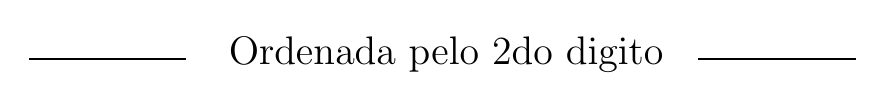
\begin{tikzpicture}
        \draw[thick] (0,0) -- (2,0); % Línea antes del texto
        \node[anchor=mid] at (5.3,0) {\Large Ordenada pelo 2do digito}; % Texto centrado
        \draw[thick] (8.5,0) -- (10.5,0); % Línea después del texto
    \end{tikzpicture}
\end{center}
\begin{center}
    s\textcolor{red}{e}a, t\textcolor{red}{e}a, m\textcolor{red}{o}b, t\textcolor{red}{a}b, d\textcolor{red}{o}g, r\textcolor{red}{u}g, d\textcolor{red}{i}g, b\textcolor{red}{i}g, \\
    b\textcolor{red}{a}r, e\textcolor{red}{a}r, t\textcolor{red}{a}r, c\textcolor{red}{o}w, r\textcolor{red}{o}w, n\textcolor{red}{o}w, b\textcolor{red}{o}x, f\textcolor{red}{o}x
\end{center}
\[
C = \quad
\begin{array}{|c|}
\hline
a \\ \hline
b \\ \hline
c \\ \hline
d \\ \hline
e \\ \hline
f \\ \hline
g \\ \hline
h \\ \hline
i \\ \hline
j \\ \hline
k \\ \hline
l \\ \hline
m \\ \hline
n \\ \hline
o \\ \hline
p \\ \hline
q \\ \hline
r \\ \hline
s \\ \hline
t \\ \hline
u \\ \hline
v \\ \hline
w \\ \hline
x \\ \hline
y \\ \hline
z \\ \hline
\end{array}
\quad
\begin{minipage}{6cm}
\raggedright % Alinea el texto a la izquierda
bar, ear, tar, tab\\%a
-\\%b
-\\%c
-\\%d
tea, sea\\%e
-\\%f
-\\%g
-\\%h
dig, big\\%i
-\\%j
-\\%j
-\\%k
-\\%l
-\\%m
%-\\%n
box, fox, cow, row, now, dog, mob\\%o
-\\%p
-\\%q
-\\%r
-\\%s
-\\%t
rug\\%u
-\\
-\\%v
-\\%w
-\\%x
-\\%y
-\\%z
\end{minipage}
\]
\begin{center}
    tab, tar, ear, bar, sea, tea, big, dig,\\
    mob, dog, now, row, cow, fox, box, rug
\end{center}

\begin{center}
    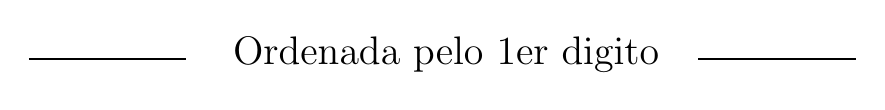
\begin{tikzpicture}
        \draw[thick] (0,0) -- (2,0); % Línea antes del texto
        \node[anchor=mid] at (5.3,0) {\Large Ordenada pelo 1er digito}; % Texto centrado
        \draw[thick] (8.5,0) -- (10.5,0); % Línea después del texto
    \end{tikzpicture}
\end{center}
\begin{center}
    \textcolor{red}{t}ab, \textcolor{red}{t}ar, \textcolor{red}{e}ar, \textcolor{red}{b}ar, \textcolor{red}{s}ea, \textcolor{red}{t}ea, \textcolor{red}{b}ig, \textcolor{red}{d}ig,\\
    \textcolor{red}{m}ob, \textcolor{red}{d}og, \textcolor{red}{n}ow, \textcolor{red}{r}ow, \textcolor{red}{c}ow, \textcolor{red}{f}ox, \textcolor{red}{b}ox, \textcolor{red}{r}ug
\end{center}
\[
C = \quad
\begin{array}{|c|}
\hline
a \\ \hline
b \\ \hline
c \\ \hline
d \\ \hline
e \\ \hline
f \\ \hline
g \\ \hline
h \\ \hline
i \\ \hline
j \\ \hline
k \\ \hline
l \\ \hline
m \\ \hline
n \\ \hline
o \\ \hline
p \\ \hline
q \\ \hline
r \\ \hline
s \\ \hline
t \\ \hline
u \\ \hline
v \\ \hline
w \\ \hline
x \\ \hline
y \\ \hline
z \\ \hline
\end{array}
\quad
\begin{minipage}{6cm}
\raggedright % Alinea el texto a la izquierda
-\\%a
box, big, bar\\%b
cow\\%c
dog, dig\\%d
ear\\%e
fox\\%f
-\\%g
-\\%h
-\\%i
-\\%j
-\\%j
-\\%k
-\\%l
mob\\%m
now\\%n
-\\%o
-\\%p
-\\%q
rug, row\\%r
sea\\%s
tea, tar, tab\\%t
-\\%u
-\\
-\\%v
-\\%w
-\\%x
-\\%y
-\\%z
\end{minipage}
\]
\begin{tcolorbox}[title=Resposta, colframe=black, colback=white] % Personaliza el color del marco y del fondo
    bar, big, box, cow, dig, dog, ear, fox, 
    mob, now, row, rug, sea, tab, tar, tea
\end{tcolorbox}

\subsection {(0,4) Dentre todos os algoritmos de ordenação vistos até o momento, quais seriam os
mais eficientes (considerando tempo de execução e uso de memória) para cada caso,
explique sua escolha:}

\subsubsection {3.a. Uma lista ordenada em ordem ascendente}

De acordo com os testes que realizei em uma pratica anterior da disciplina para um array ordenado ascendente de 1000 elementos, o algoritmo que me deu melhor tempo en segundos foi o Shellsort, 
mas se olharmos para o lado da complexidade e a teoria nos disser que o algoritmo Insertion Sort é o mais eficiente neste caso, com complexidade 
$O(n)$, pois só verificaria se a lista já está ordenada. Outros algoritmos, como Quicksort ou Mergesort, mantêm sua complexidade 
$O(nlogn)$.



\subsubsection {3.b. Uma lista ordenada em ordem descendente}
De acordo com os testes que realizei em uma pratica anterior da disciplina para um array ordenado descendente de 1000 elementos, o algoritmo que me deu melhor tempo en segundos foi o Shellsort, 
mas se olharmos só a complexidade e a teoria o algoritmo
Quicksort é eficiente com $O(nlogn)$ na média, mas pode ser pior em alguns casos (
$O(n^2)$). Tambem se tem o Heapsort que a diferença do Quicksort, ele sempre tem $O(nlogn)$ no pior caso.

\subsubsection {3.c. Uma lista com os valores desordenados aleatoriamente}

Quicksort é um dos mais eficientes na média, com $O(nlogn)$, seguido por Heapsort e Mergesort, ambos com a mesma complexidade.

\subsubsection {3.d. Elementos com valores iguais não sejam trocados de ordem (estável).}

Mergesort e Counting Sort são estáveis, ou seja, mantêm a ordem relativa dos elementos com valores iguais, com complexidades 
$O(nlogn)$ e $O(n+k)$, respectivamente.

\end{document}